\section{Theory}
\label{sec:theory}
Since we want to highlight the historical importance of the discovery of the Compton effect, we introduce the theoretical 
backgrounds in close relation to the questions asked at the beginning of the last century. Taking this perspective, we 
review the theories existing prior to Compton's explanation and their points of failure. His "new" quantum mechanical 
approach yielded two central results: the prediction of a shift in wavelength and a cross section dependent on the 
wavelength of the incident radiation. Both features are described on the following pages. 

\subsection{Failure of Thomson scattering}
\label{sec:thomson}
At the beginning of the 1920s, the nature of electromagnetic radiation was still subject of a large debate within the 
physics community. Although Einstein had shown the particle-like character of light in case of the photoelectric effect, 
this picture was nowhere near being widely accepted. Instead, most theories based on classical electrodynamics and people 
were using quite complicated deviations in order to stay with the classic theory. Reading Compton's original paper, one is 
confronted with a vivid description of these seemingly desperate attempts.\cite{compton} 
To understand these difficulties, we introduce the 
theory of Thomson scattering, a classical description of elastic scattering of electromagnetic radiation at charged 
particles. In our case, we deal with electrons. These are accelerated by the electric field and will thus act as Hertzian 
dipoles. They emit radiation of the same frequency as the incident rays, in terms of wavelength:
\begin{equation}
    \lambda_\text{Th}' - \lambda = 0\, ,	
    \label{eq:thomsom_lamb}
\end{equation}
where $\lambda$ denotes the wavelength of the incident radiation and $\lambda_\text{Th}'$ the one of the scatter rays.
For radiation of low frequency (soft X-rays and lower), this had been successfully tested experimentally. However, for 
hard X-rays and $\gamma$-rays, the observations were contradictory: The wavelength of scattered light was higher. Compton 
previously tried to ascribe this to fluorescence, but after conducting his experiment, he found it "difficult to attribute
it to anything other then true scattering"\cite{compton}. 

The second substantial disagreement between the acquired experimental data and Thomson's theory was the cross section of 
the scattering in the regime of hard X-rays and $\gamma$-rays. The classical theory yields a cross section independent of 
the wavelength of incident radiation. The differential cross section dependent on the scattering angle $\theta$ is given by
\begin{equation}
    \begin{split}
        \frac{\text{d} \sigma_\text{Th}}{\text{d} \Omega} 
        &= \frac{1}{2} \left(\frac{e^2}{m_e c^2}\right)^2 \left(1 + \cos^2 \theta  \right)  \\
        &= \frac{1}{2} r_e^2 \left(1 + \cos^2 \theta  \right) 
        \label{eq:thomson}
    \end{split}
\end{equation}
with the classical electron radius $r_e = e^2/m_e c^2$. 
The total cross section is then calculated by integrating over the entire sphere:
\begin{equation}
    \begin{split}
        \sigma_\text{Th, total} &= \int_\Omega \! \frac{\text{d} \sigma_\text{Th}}{\text{d} \Omega}  \, \text{d}\Omega \\
            &= \left(\frac{1}{2} r_e^2\right)  2\pi \int_0^\pi \! \left(1 + \cos^2\theta\right)\sin\theta \, \text{d}\theta \\
            &= r_e^2\pi \left[ -\cos\theta -\frac{1}{3}\cos^3\theta \right]_0^\pi \\
            &= \frac{8\pi}{3} r_e^2 
        \label{eq:total_thomson}
    \end{split}
\end{equation}
Inserting the numerical values, we get a cross section of $\sigma_\text{Th, total} = 66.524 \text{ fm}^2$. 
However, in the regime in question the cross section turned out to be considerably lower. An idea put forward prior to 
1923 was the "large electron", having a radius comparable to that of the wavelength of X-rays or $\gamma$-rays. Compton's
experiment wrecked these attempts because it turned out that the radius would have to adapt to the wavelength of the 
radiation.\cite{compton}   

A third difficulty of the classical theory was the description of the discrete nature of scattering events in the case of 
low intensity incident radiation. Today, this is of course interpreted from the perspective of photons being discrete 
quanta of light. In the classical theory, however, one assumed a continuous electrical field acting on the entire sample
with the scattered radiation as a result of interference. 

Notwithstanding all these problems, Thomson's theory remains an important tool e.~g. in plasma physics, as it turns out to
be the limit of th quantum mechanical description in the regime of low energy, essentially for incident frequencies 
$\nu \ll \frac{m_ec^2}{h}$. At this point, nonetheless, we will turn back to our central subject which overcame all of the
stated problems and had a large influence on the following change in paradigm. 

\subsection{Shift in wavelength}
\label{sec:wavelength}
Compton's picture in order to explain the observed phenomena was that of a elastic scattering between a quasi-free electron
and an incident photon. A sketch of this situation in the rest frame of the electron is shown in 
figure~\ref{fig:compton_scatter}. With this picture, the assumption of the conservation of energy \textit{and} momentum 
becomes natural. In the following, we use this axiomatic approach to derive and expression for the difference in
wavelength $\lambda' - \lambda$ at angle $\theta$. Energy conservation reads 
\begin{equation}
    E_ = 	
    \label{eq:energy_conservation}
\end{equation}




\begin{figure}[htpb]
    \centering
    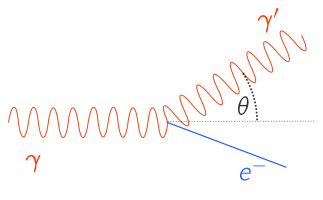
\includegraphics[width=0.8\linewidth]{figures/compton_scatter}
    \caption{
        Scheme of Compton scattering in the rest frame of the electron prior to the scattering event. The photon before and
        after the scattering are distinguished by $\gamma$ and $\gamma'$ respectively. 
        }
    \label{fig:compton_scatter}
\end{figure}


\subsection{Cross section}
\label{sec:cross_section}


\subsection{BKS}
\label{sec:BKS}

